\documentclass[hyphens,aspectratio=169,dvipsnames]{beamer}
\usepackage{graphicx}
\usepackage{xcolor}
\usepackage{amssymb}
\usepackage{amsmath}
\usepackage{mathtools}
\usepackage{textcomp}
\usepackage{moresize}
\usepackage{framed}
\usepackage{minted}
\usepackage{relsize}
\usepackage{tikz}
\usepackage{comment}
\usetikzlibrary{shapes.geometric, arrows, positioning}
\usetheme{Berlin}
\usecolortheme[RGB={0,95,47}]{structure}
\beamertemplatenavigationsymbolsempty

\makeatletter
\AtBeginEnvironment{minted}{\dontdofcolorbox}
\def\dontdofcolorbox{\renewcommand\fcolorbox[4][]{##4}}
\makeatother

\newcommand{\textpf}[1]{\texttt{\color{black}\fcolorbox{lightgray}{lightgray}{#1}}}

\begin{document}

\begin{frame}{CPU Privelege Levels}
    \begin{itemize}
        \pause \item x86\_64 CPUs have two primary privilege levels: ring 0 (kernel) and ring 3 (user).
        \pause \item When a CPU is executing in ring 3, it is in its least priveleged state.
        \pause \item When a CPU is executing in ring 0, it is in its most priveleged state.
    \end{itemize}
\end{frame}

\begin{frame}{}
    \begin{center}
        \begin{tabular}{c c}
            Ring 3 & Ring 0 \\
            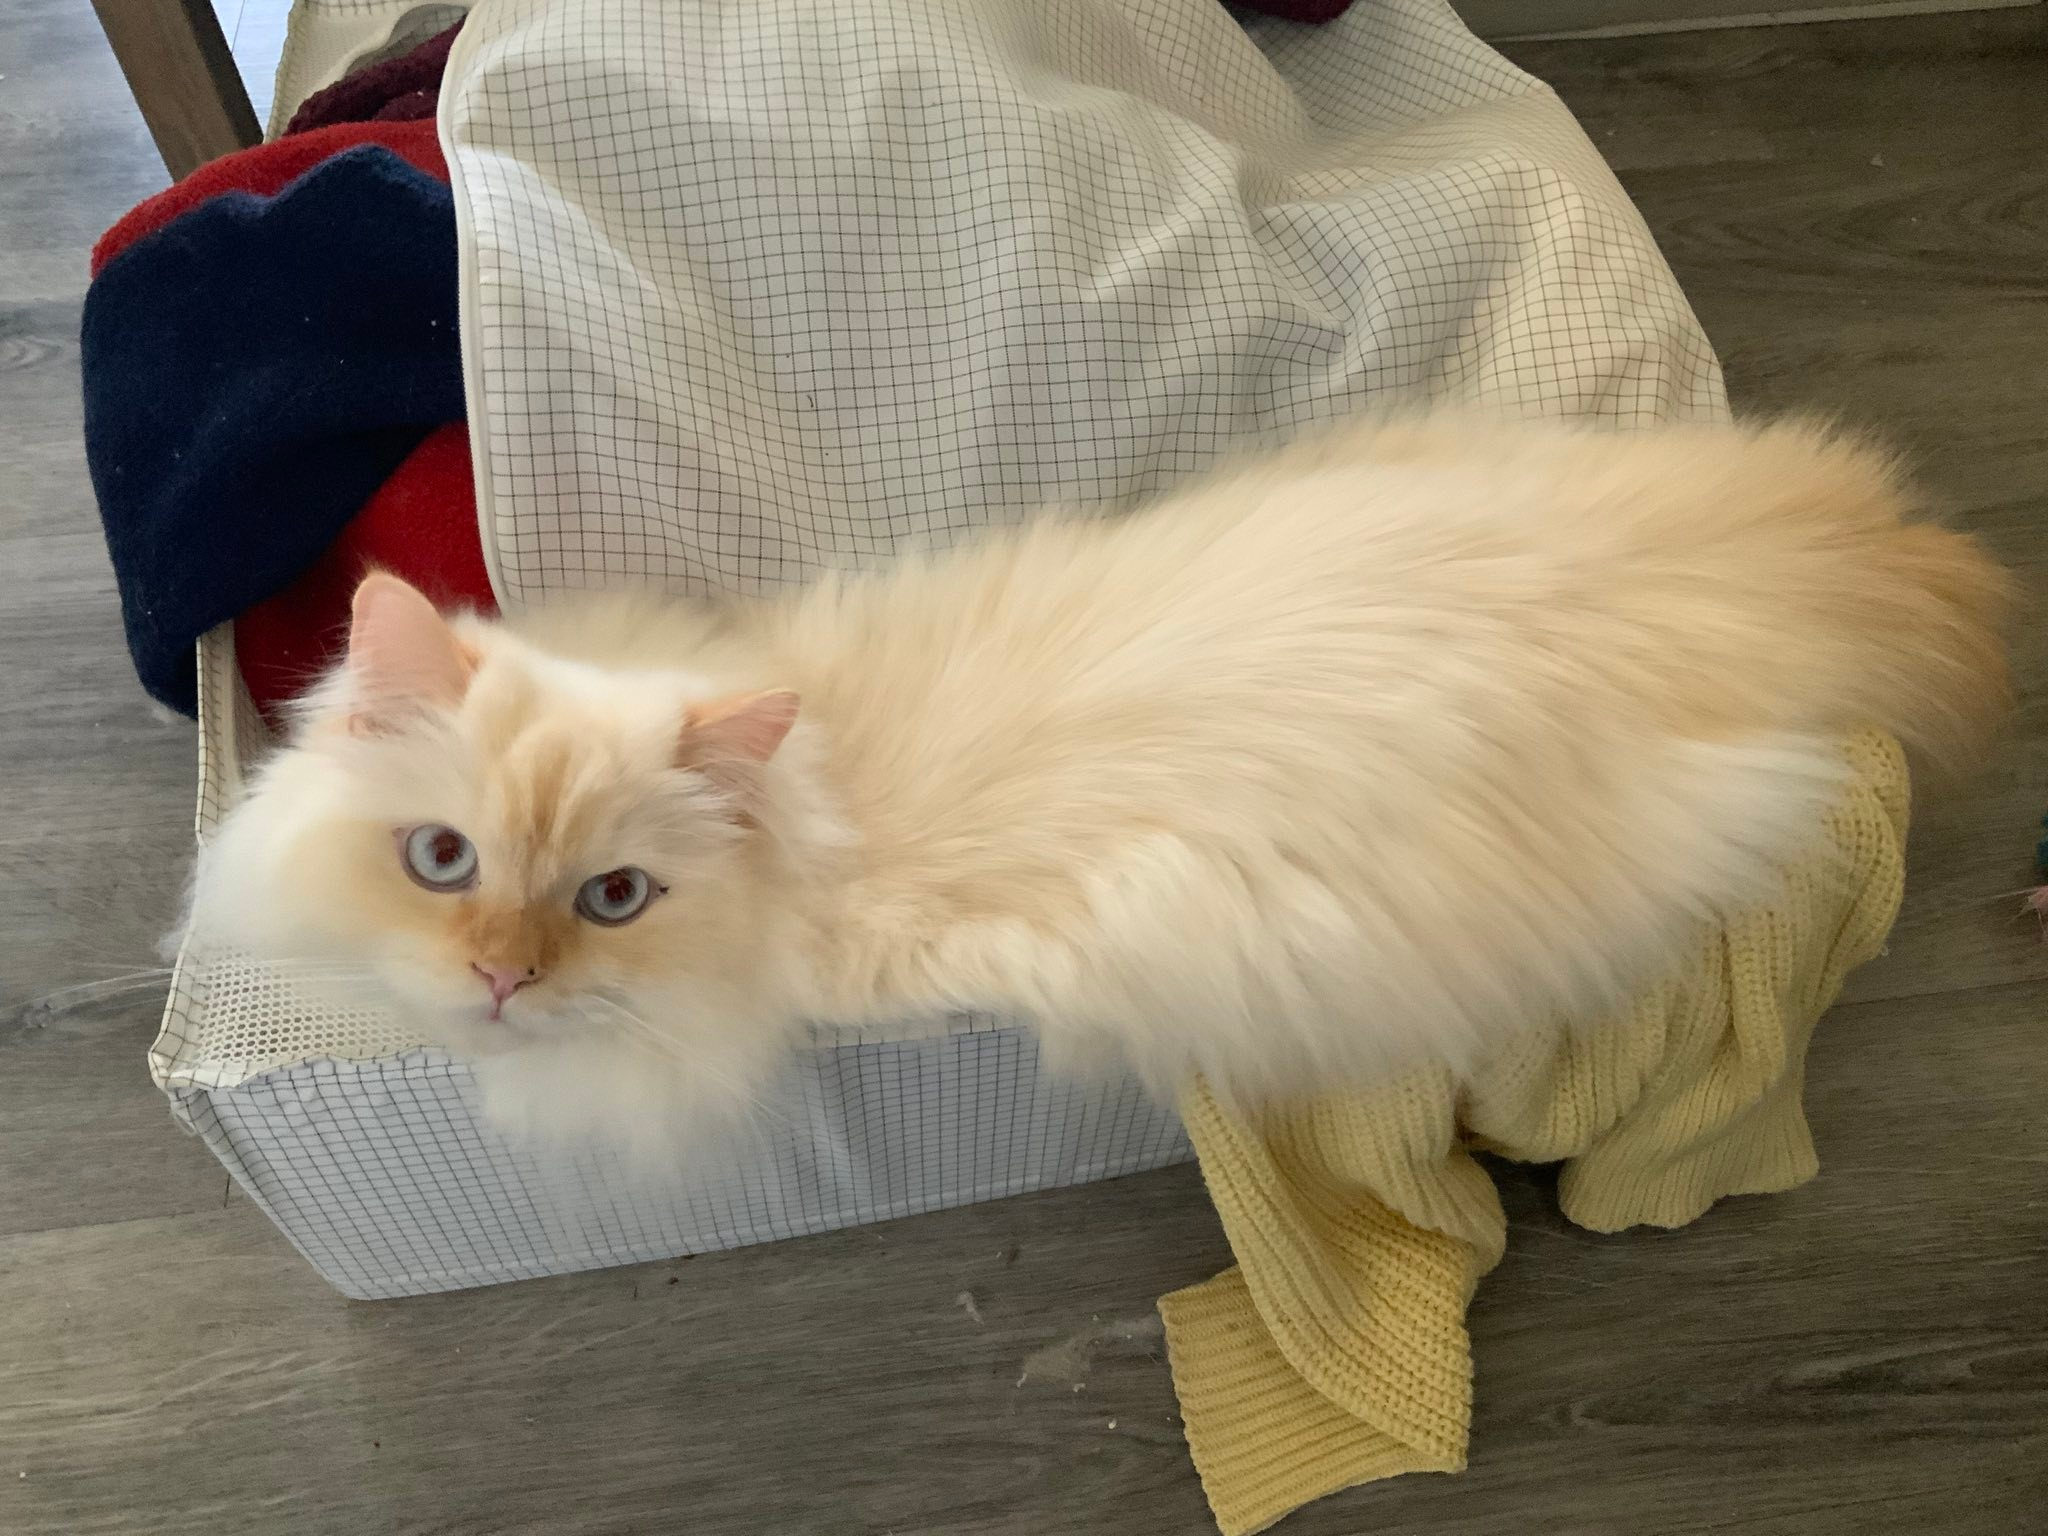
\includegraphics[height=0.3\textwidth]{davey.jpeg} & 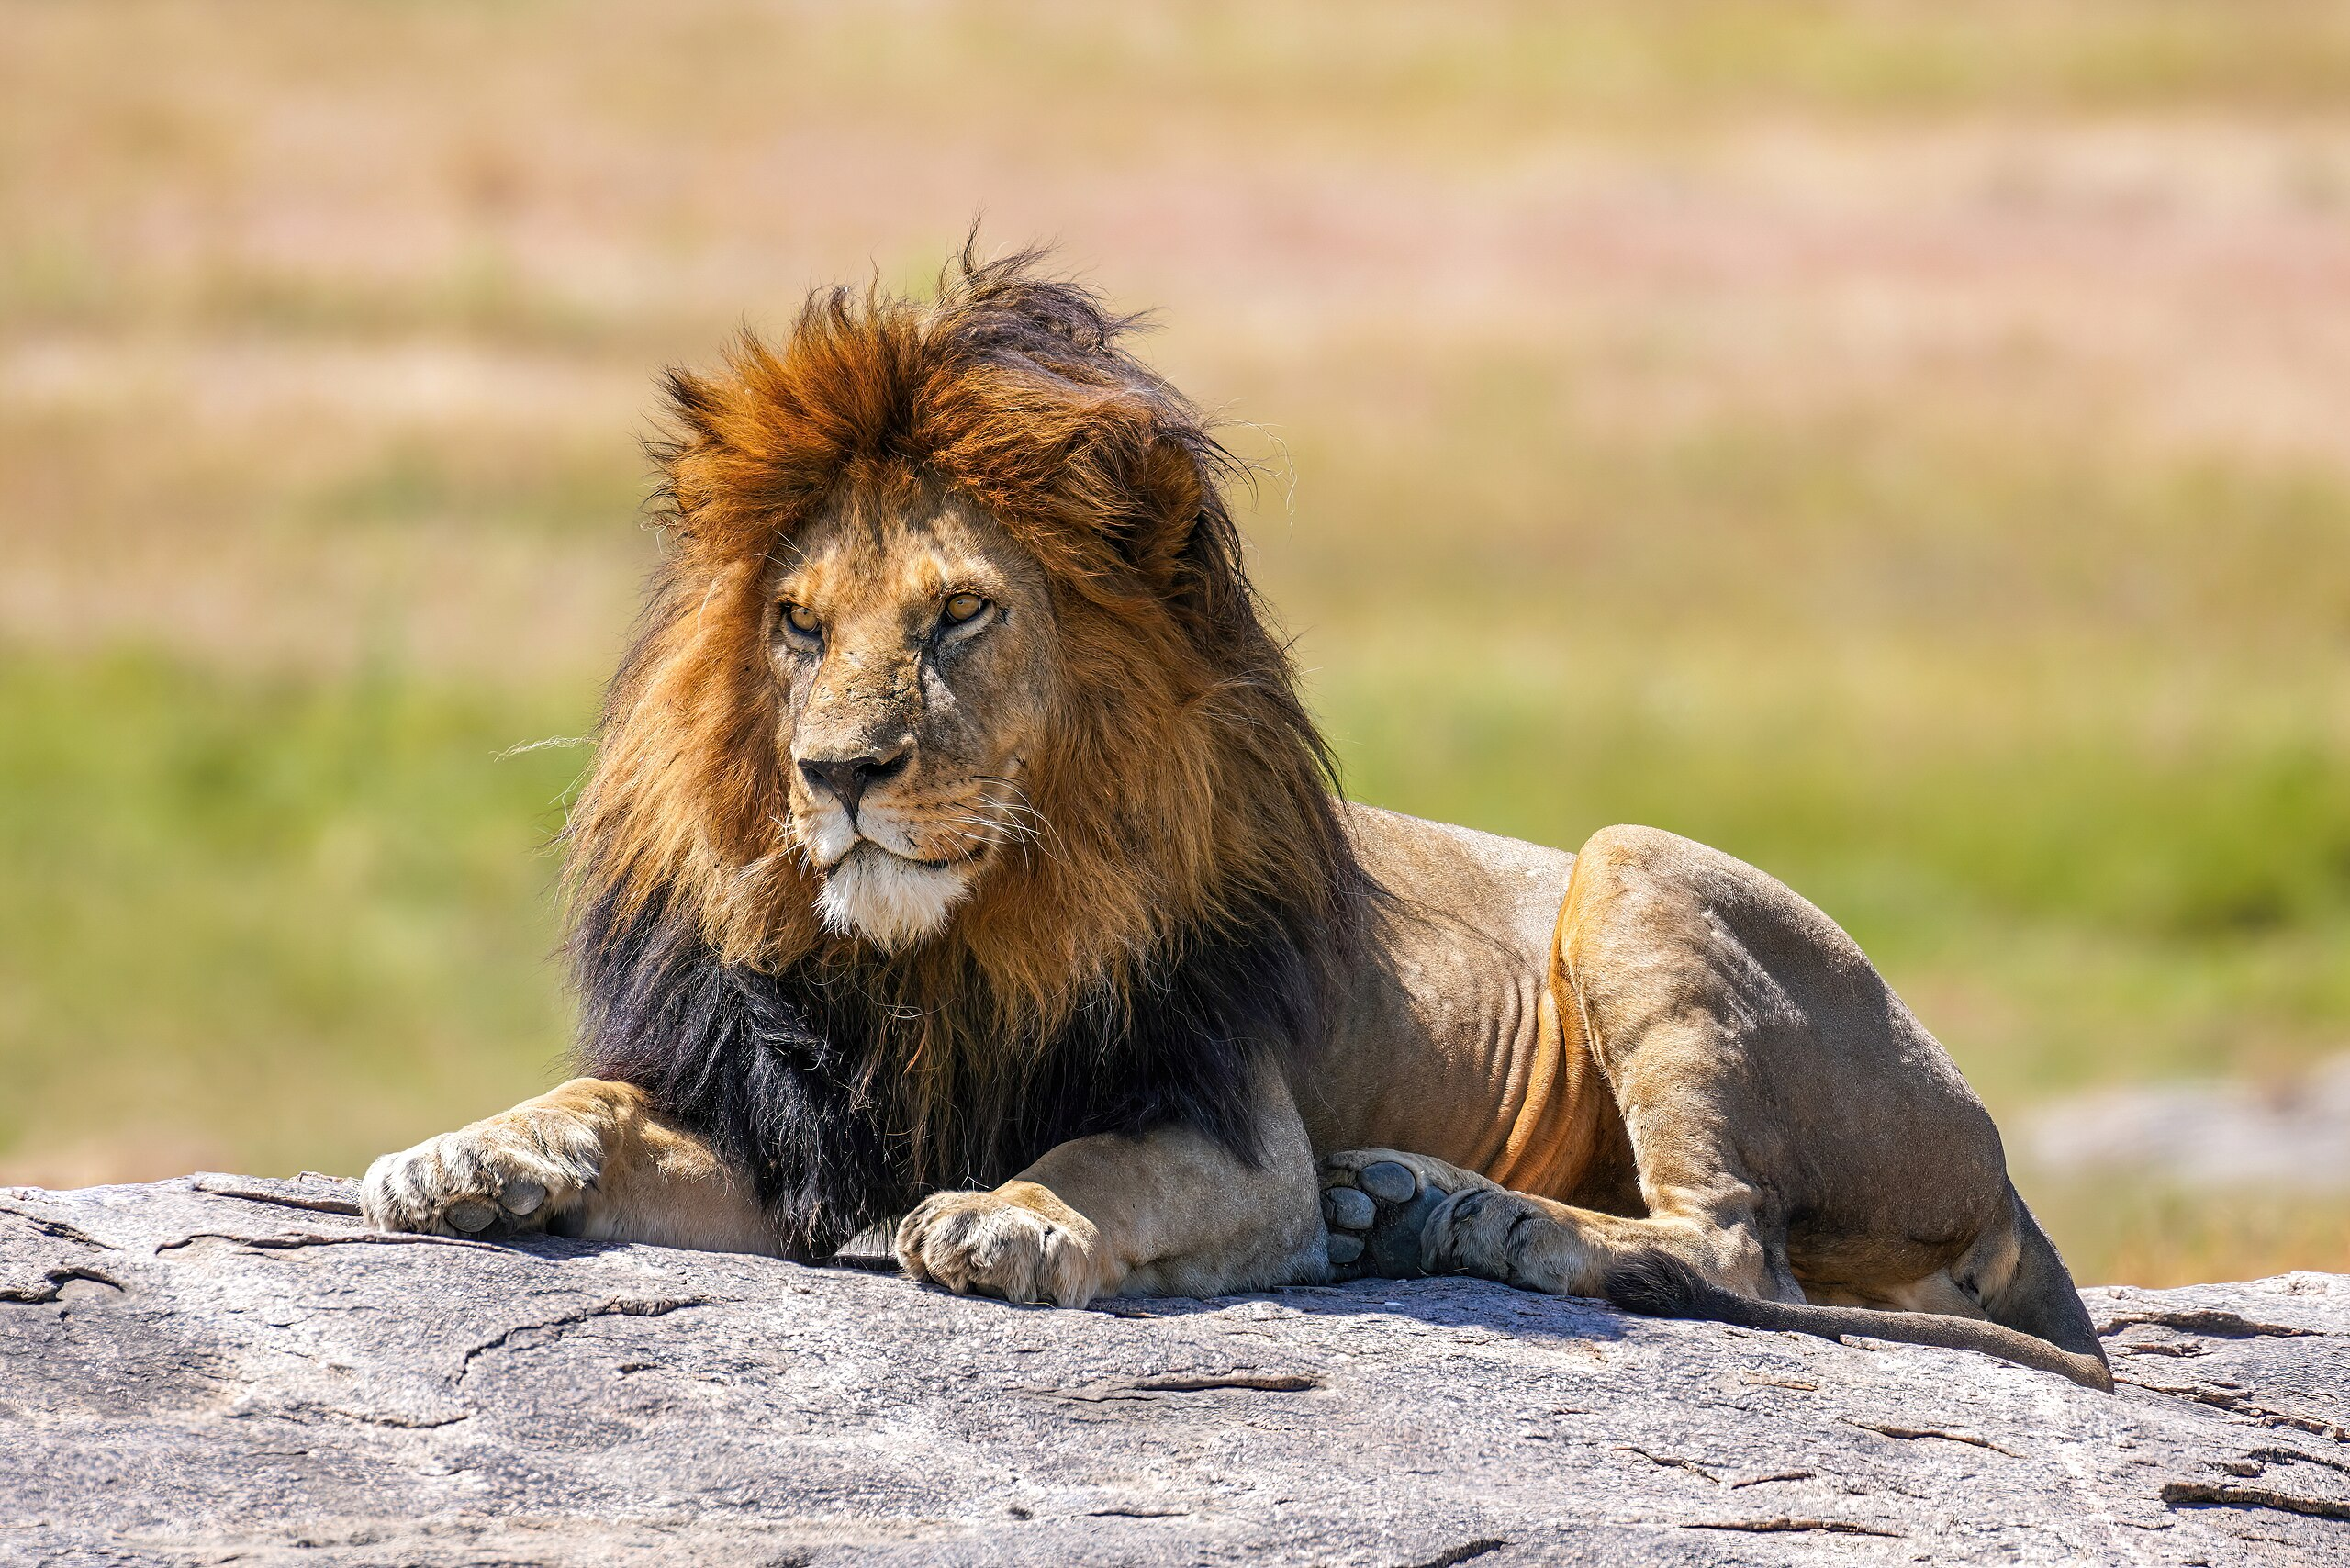
\includegraphics[height=0.3\textwidth]{lion.jpg}
        \end{tabular}
    \end{center}
\end{frame}

\begin{frame}{Ring 3}
    \begin{itemize}
        \pause \item All the code you have ever run on an x86\_64 CPU has been in ring 3.
        \pause \item Even when you're \texttt{root}, you're still in ring 3.
    \end{itemize}
\end{frame}

\begin{frame}{Ring 0}
    Much of the interesting stuff that computers do can only be done from ring 0.
    This includes
    \begin{itemize}
        \pause \item Sending/receiving data over the network
        \pause \item Reading/writing to/from files
        \pause \item Printing stuff to \textpf{stdout}
        \pause \item Interacting with peripherals
    \end{itemize}
\end{frame}

\begin{frame}{Accessing Ring 0 from Ring 3}
    \begin{itemize}
        \pause \item If all those things require ring 0 privileges, and your code runs in ring 3, how is your code able to do those things?
        \pause \item System calls!
    \end{itemize}
\end{frame}

\begin{frame}{System Calls}
    \begin{itemize}
        \pause \item System calls (a.k.a. syscalls) are how user programs ask the kernel to do privileged operations.
        \pause \item Each syscall has a unique \textit{syscall number}.
    \end{itemize}

    For example,
    \begin{itemize}
        \pause \item The \texttt{read} syscall (x86\_64 syscall number 0) reads from a file descriptor.
        \pause \item The \texttt{write} syscall (x86\_64 syscall number 1) writes to a file descriptor.
        \pause \item The \texttt{execve} syscall (x86\_64 syscall number 59) executes a new program, overwriting the currently running process.
        \pause \item The \texttt{exit} syscall (x86\_64 syscall number 60) exits the process.
    \end{itemize}
\end{frame}

\begin{frame}{Making a System Call}
    \begin{itemize}
        \pause \item To make a system call, use the \textpf{syscall} libc function, provided by \textpf{<unistd.h>}.
        \pause \item The first argument to this function is the syscall number of the system call you'd like to invoke.
        \pause \item The rest of the arguments depend on which system call you're invoking.
        \pause \item Consult this giant table for more details:
        \pause \item \url{https://www.chromium.org/chromium-os/developer-library/reference/linux-constants/syscalls/}
    \end{itemize}
\end{frame}

\end{document}
